\documentclass{article}
\bibliographystyle{plain}
\linespread{1.2}
\usepackage[margin = 1.25 in]{geometry}
\usepackage{wrapfig}
\usepackage{amsfonts}
\usepackage[utf8]{inputenc}
\usepackage[T1]{fontenc}
\usepackage{graphicx}
\usepackage[english]{babel}
\usepackage[algoruled]{algorithm2e}

\renewcommand{\theequation}{\thesection.arabic{equation}}

\renewcommand{\thefigure}{\thesection.\arabic{figure}}



\renewcommand{\vec}[1]{\mathbf{#1}}
\renewcommand{\theequation}{\thesubsection.\arabic{equation}}
\DeclareGraphicsExtensions{.pdf,.png,.jpg, .gif}

\usepackage{amsthm}

\usepackage[english]{babel}
\usepackage{mathtools}

%\usepackage[OT2,T1]{fontenc}
%\DeclareSymbolFont{cyrletters}{OT2}{wncyr}{m}{n}
%\DeclareMathSymbol{\sha}{\mathalpha}{cyrletters}{"58}

\DeclareFontFamily{U}{wncy}{}
\DeclareFontShape{U}{wncy}{m}{n}{<->wncyr10}{}
\DeclareSymbolFont{mcy}{U}{wncy}{m}{n}
\DeclareMathSymbol{\Sh}{\mathord}{mcy}{"58} 
\DeclareMathOperator*{\argmin}{arg\,min}

\newcounter{eqn}
\renewcommand*{\theeqn}{\alph{eqn})}
\newcommand{\num}{\refstepcounter{eqn}\text{\theeqn}\;}

\makeatother
\newcommand{\vectornorm}[1]{\left|\left|#1\right|\right|}
\newcommand*\conjugate[1]{\bar{#1}}

\newtheorem{thm}{Theorem}
\newtheorem{defn}{Definition}
 %\theoremstyle{plain}
  \newtheorem{theorem}{Theorem}[section]
  \newtheorem{corollary}[theorem]{Corollary}
  \newtheorem{proposition}[theorem]{Proposition}
  \newtheorem{lemma}[theorem]{Lemma}
\newtheorem{example}[theorem]{Example}
  \newtheorem{definition}[theorem]{Definition}
  \newtheorem{conj}[theorem]{Conjecture}
 \newtheorem{condition}{Condition}
 \newtheorem{remark}[theorem]{Remark}

\newcommand{\supp}{\operatorname{supp}} 
\newcommand{\vc}[1]{{\mathbf{ #1}}}
\newcommand{\tn}{\widetilde{\nabla}_{n} }
\newcommand{\Z}{{\mathbb{Z}}}
\newcommand{\re}{{\mathbb{R}}}
\newcommand{\II}{{\mathbb{I}}}
\newcommand{\ep}{{\mathbb{E}}}
\newcommand{\pr}{{\mathbb{P}}}
\newcommand{\FF}{{\mathcal{F}}}
\newcommand{\TT}{{\mathcal{T}}}
\newcommand{\phin}{\phig{n}}
\newcommand{\phig}[1]{\phi^{(#1)}}
\newcommand{\ol}[1]{\overline{#1}}
\newcommand{\eff}{{\rm eff}}
\newcommand{\suc}{{\rm suc}}
\newcommand{\tends}{\rightarrow \infty}
\newcommand{\setS}{{\mathcal{S}}}
\newcommand{\setP}{{\mathcal{P}}}
\newcommand{\setX}{{\mathcal{X}}}
\newcommand{\nec}{{\rm nec}}
\newcommand{\bd}{{\rm bd}}

\title{New Basis}

\begin{document}
\maketitle

\section{Preliminaries}
Consider the basis defined by the function:

\begin{equation}
f_i\left(x\right) =
\begin{cases}
1 & \text{if } x \leq i \\
0 & \text{ otherwise } 
\end{cases}
\label{basis}
\end{equation}

That is, \(f_i\) is a left-hand step function. We define the inner product between two vectors as follows:

\begin{definition}
\begin{equation}
\langle x, y \rangle = x^T y = \sum_i x_i y_i
\end{equation}	
where \(x_i, y_i\) are the components of the vectors \(x,y\) in the \(i^{th}\) direction with respect to some basis vectors \(e_i\).
\end{definition}

We can define a matrix representation for the set of basis vectors \(f_i\), by taking all inner products between all pairs basis vectors:

\begin{definition}
\begin{equation}
F_{n, ij} = \langle f_i, f_j \rangle
\end{equation}

This matrix has the representation:

\begin{equation}
F_{ij} = min(i,j)
\end{equation}

An example of such a matrix is:

\begin{equation}
F_n= \begin{pmatrix}
 1 & 1 & 1 & 1  & 1 \\
  1 & 2 & 2 & 2  & 2\\
     1 & 2 & 3 & 3  & 3  \\
    1 & 2 & 3 & 4  & 4  \\
     1 & 2 & 3 & 4  & 5 
\end{pmatrix}
\end{equation}
\end{definition}

This matrix is invertible.

\begin{theorem}
\begin{equation}
det(F_n) = 1
\end{equation}
\end{theorem}
\begin{proof}
Consider the matrix \(F^n\). Subtract the \(n-1\)th column from the \(n\)th. We obtain a matrix with \(0\) on the final column except the entry \(F^n_(n,n) = 1\). Since the top \((n-1) \times (n-1)\) is \(F^{n-1}\) we find that 

\begin{equation}
det(F_n) = 1 \times det(F_{n-1})
\end{equation} 

By recursion and \(det(F_1) = 1\) we have \(det(F_n) = 1\).

\end{proof}

This matrix can be factorised as \(F = LL^T\) where 

\begin{equation}
L = \begin{pmatrix}
 1 & 0 & 0 & 0  & 0 \ldots 0 \\
  1 & 1 & 0 & 0  & 0 \ldots 0\\
     1 & 1 & 1 & 0  & 0 \ldots0  \\
    \ldots  \\
     1 & 1 & 1 & 1  & 1 \ldots 1 
\end{pmatrix}
\end{equation}

From this it follows that

\begin{equation}
F^{-1} = \begin{pmatrix}
 2 & -1 & 0 & 0  & 0 \ldots 0 \\
  -1 & 2 & -1 & 0  & 0 \ldots 0\\
     0 & -1 & 2 & -1  & 0 \ldots0  \\
    \ldots  \\
     0 & 0 & 0 & 0  \ldots -1 & 1 
\end{pmatrix}
\end{equation}

Another matrix we will use a lot of is:

\begin{equation}
D = \begin{pmatrix}
 1 & 0 & 0 & 0  & 0 \ldots 0 \\
  -1 & 1 & 0 & 0  & 0 \ldots 0\\
     0 & -1 & 0 & 0  & 0 \ldots0  \\
    \ldots  \\
     0 & 0 & 0 & 0  \ldots -1 & 1
\end{pmatrix}
\end{equation}

and by direct computation:

\begin{equation}
DL = I
\label{Dinv}
\end{equation}

\section{Spectrum Sensing}

We model our PSD signal \(g\) as a linear combination of the basis functions (\ref{basis}):

\begin{equation}
g\left(x\right) = \sum_i a_i f_i 
\label{basis-expansion}
\end{equation}

To find the \(a_i\), we correlate (take the inner product of) the signal against the basis (\ref{basis}).

\begin{definition}
\begin{align}
h_j &= \langle g, f_j \rangle \\
&= \sum_j g\left(x\right) f_j\left(x\right) \\
&= \sum_j a_i f_i\left(x\right) f_j\left(x\right) \\
&= a_i \langle f_i, f_j\rangle \\
&\left(= \sum_{x=1}^j g\left(x\right)\right)
\end{align}

In matrix language \(h = F a^T\). This is the inner product between the signal \(g\) and the basis functions \(f_i\).
\end{definition}

\begin{definition}
\begin{equation}
d_i\left(x\right) =
\begin{cases}
1 & \text{if } x = i \\
-1 & \text{if } x = i-1 \\
0 & \text{otherwise} 
\end{cases}
\end{equation}
i.e. \(d_i\) is the \(i^{th}\) row of the matrix \(D\).
\end{definition}

\begin{theorem}
\begin{equation}
D^Tg = a
\end{equation}
\end{theorem}
\begin{proof}
From the definition of \(g\) (\ref{basis-expansion})

\begin{align}
D^Tg &= D^T \sum_i a_i f_i \\
&= \sum_i a_i d_j^T f_i \\
&= a \langle d_j, f_i\rangle \\
&= a
\end{align}
as
\begin{equation}
\langle d_j, f_i \rangle = =
\begin{cases}
1 & \text{if } i \leq j \\
0 & \text{otherwise} 
\end{cases}
\end{equation}
\end{proof}

This means 

\begin{equation}
g = \left(D^T\right)^{-1} a =\left(D^{-1}\right)^T a
\end{equation}

so using (\ref{Dinv}), 

\begin{equation}
g = L^T a
\end{equation}

To recover \(\hat{a}\), we minimise

\begin{equation}
\vectornorm{h - Fa}_2^2
\end{equation}

in the noiseless case, and

\begin{equation}
\vectornorm{h_\varepsilon - Fa}_2^2 + \lambda\vectornorm{a}_1
\label{recon}
\end{equation}

in the noisy case, where 

\begin{equation}
\left(h_\varepsilon\right)_j = \langle\left(g+\varepsilon\right), f_j\rangle
\end{equation}

and \(\varepsilon \sim \mathcal{N}(0,\sigma^2\ I)\).

From \(\hat{a}\) we can recover \(\hat{g}\) from the following relation:

\begin{equation}
\hat{g} = L^{T} \hat{a}
\end{equation}


\section{Results}

\begin{figure}[h]
\centering
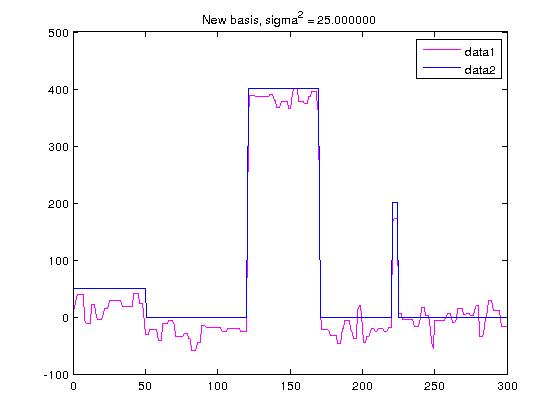
\includegraphics[height = 7.3 cm]{new_basis_25.jpg}
\caption{}
\label{fig:new_basis_25}
\end{figure}

\begin{figure}[h]
\centering
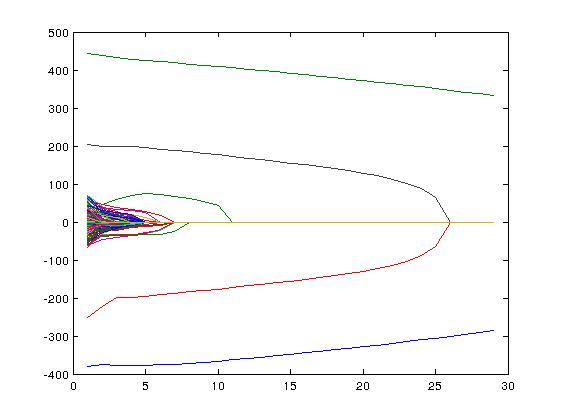
\includegraphics[height = 7.3 cm]{new_basis_different_lambdas.jpg}
\caption{}
\label{fig:new_basis_25}
\end{figure}

\begin{figure}[h]
\centering
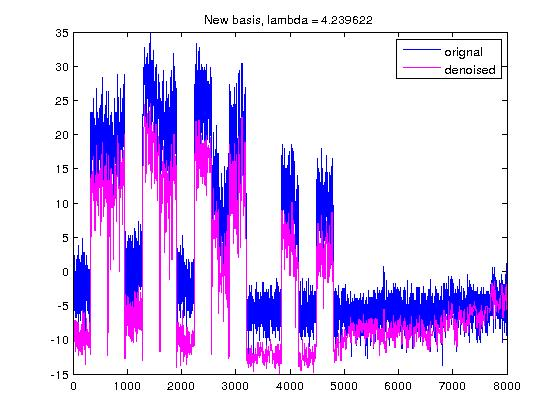
\includegraphics[height = 7.3 cm]{new_basis_ofcom_1.jpg}
\caption{}
\label{fig:new_basis_25}
\end{figure}
\begin{figure}[h]
\centering
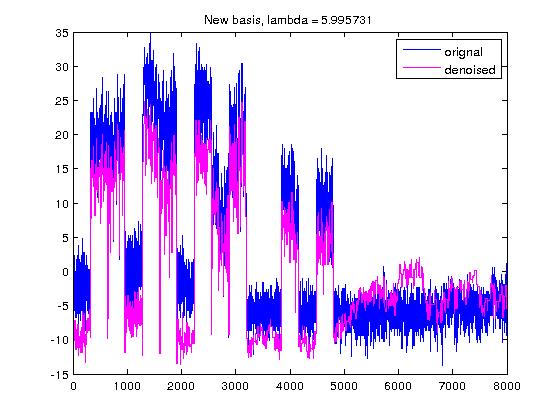
\includegraphics[height = 7.3 cm]{new_basis_ofcom_2.jpg}
\caption{}
\label{fig:new_basis_25}
\end{figure}
\begin{figure}[h]
\centering
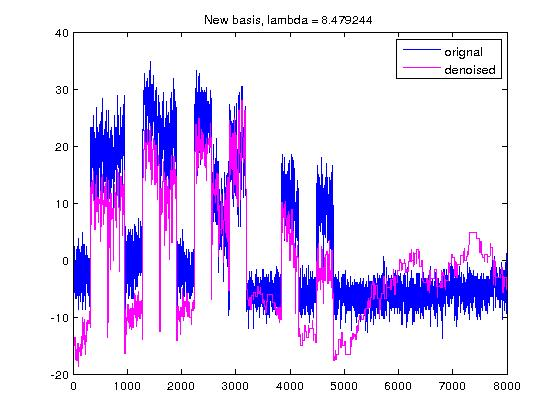
\includegraphics[height = 7.3 cm]{new_basis_ofcom_3.jpg}
\caption{}
\label{fig:new_basis_25}
\end{figure}
\begin{figure}[h]
\centering
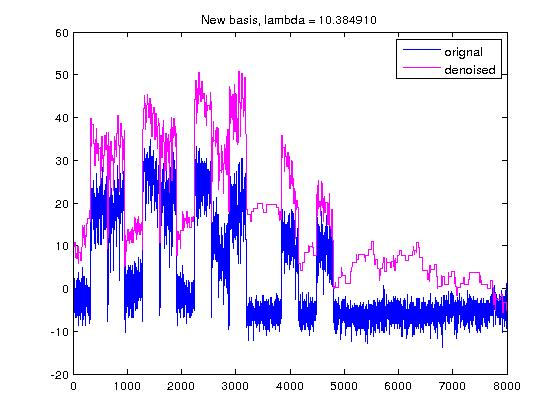
\includegraphics[height = 7.3 cm]{new_basis_ofcom_4.jpg}
\caption{}
\label{fig:new_basis_25}
\end{figure}

\begin{figure}[h]
\centering
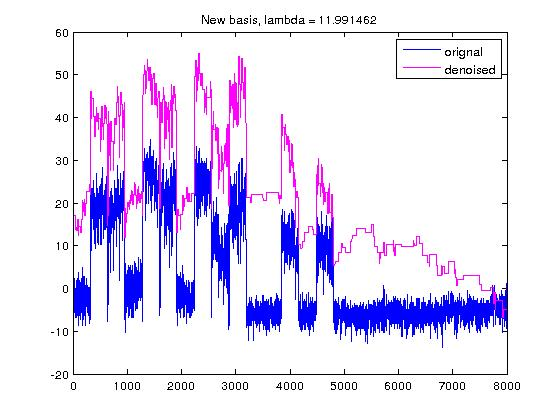
\includegraphics[height = 7.3 cm]{new_basis_ofcom_5.jpg}
\caption{}
\label{fig:new_basis_25}
\end{figure}


\end{document}